\chapter{Chapter 1. Introduction}

\section{Space Environment}
\subsection{Near-Earth solar wind}
\subsection{Interplanetary magnetic field}
%\input{Chapters/Introduction/magnetosphere}
\subsection{Bow shock}
As a spacecraft traverses near-Earth space, it moves from the solar wind through the different regimes of the terrestrial magnetosphere, the spatial domain of the magnetic-field lines that connect to the Earth \cite{Borovsky:2018}. The magnetosphere presents an obstacle to the flow of the solar wind, and as the solar wind rapidly decelerates from supersonic flow into a subsonic flow, a standing fast shock is formed upstream of Earth \cite{Dimmock:2013}. The plasma is deflected around the magnetosphere as it reaches the bow shock. The bow shock is a collisionless shock that forms from the interaction of the solar wind and Earth's magnetic field. It forms a parabolic boundary around the Earth, with the nose being approximately 15 \gls{RE} in distance in the sunward direction. However, this boundary is constantly moving due to solar wind properties. Many studies have used statistics \cite{Kruparova:2019}, machine learning techniques \cite{Lalti:2022}, or empirical models \cite{chapman_three-dimensional_2003} to identify and locate bow shock crossings of different spacecraft. The interaction of the solar wind with the bow shock can generate magnetic islands and other structures \cite{Karimabadi:2014}, and interaction with the magnetosheath leads wave generation and dissipation, magnetic reconnection, and turbulence \cite{Shaikh:2022}. %As structures and 

\subsection{Magnetosheath}
The magnetosheath is a region of shocked, turbulent, highly magnetized plasma that forms directly downstream of the bow shock. The flow of the solar wind is impeded by the Earth's magnetic field; therefore, the compressed, heated, and turbulent solar wind gets wrapped around Earth's magnetic field. This interface between Earth's terrestrial magnetosphere and the solar wind plays a significant role in the flow of particles across these boundaries. Plasma in the magnetosheath experiences large fluctuations, and \cite{Hadid:2018} estimates that the average energy cascade rate within the magnetosheath is approximately two orders of magnitude larger than the solar wind. The geometry of the bow shock and the interplanetary magnetic field determines the plasma dynamics of the magnetosheath \cite{Yordanova:2020}. Under a quasi-parallel angle of the shock normal ($<45^\circ$), the IMF is connected to the Earth's magnetic field, allowing particles to more easily enter the Earth's terrestrial magnetosphere. One such region which is under a quasi-parallel shock normal is the foreshock region, which is the region in between the last interplanetary field line that connects to the bow shock and the bow shock itself \cite{Karlsson:2021}. In the foreshock region, many solar wind particles are reflected by the bow shock, causing instabilities and other upstream phenomena, which in turn creates intense wave activity \cite{turc_transmission_2023}, such as fast magnetosonic waves \cite{Fuselier:1994}. Under a quasi-perpendicular angle of the shock normal ($>45^\circ$), the plasma experiences a sharp decrease in the velocity and sharp increase in the magnitude of the magnetic field. The temperature anisotropy is typically larger in the quasi-perpendicular region, and the quasi-perpendicular region has lower energy flux than the quasi-parallel region \cite{Gurchumelia:2022}. This turbulent layer of plasma is bounded by the magnetopause, which is the outer boundary that separates the solar wind from the magnetosphere. 

\subsection{Magnetopause}
The magnetopause is the boundary at which the solar wind pressure is equal to the dynamic pressure of Earth's magnetic field \cite{Shue:1997}. Because the pressure is not static, the magnetopause boundary moves in relation to the solar wind properties. The standoff distance of the magnetopause nose can be estimated by taking the solar wind ram pressure and setting it equal to the magnetic pressure of Earth's magnetic field. This distance is typically 6-15 $R_E$, based on solar wind conditions \cite{Collado-Vega:2023}. Figure \ref{fig:magnetopause} shows an overview of the bow shock and magnetopause boundaries, as well as a representation of the flow of plasma (black arrows). 

\begin{figure}
    \centering
    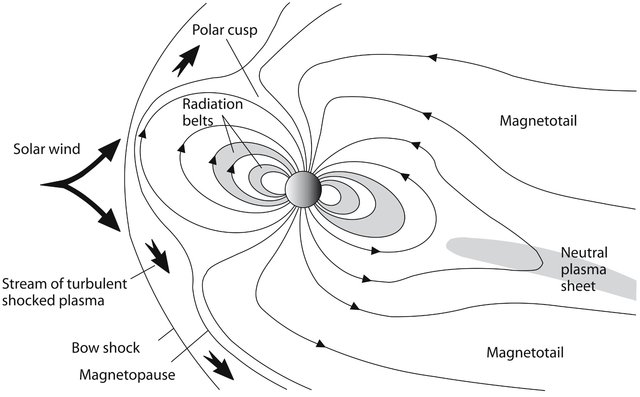
\includegraphics[width=\linewidth]{Figures/The-magnetosphere-is-the-region-where-Earths-magnetic-field-predominates-The_W640.jpg}
    \caption[Diagram of the magnetopause and Earth's magnetic field lines.]{Diagram of the magnetopause and Earth's magnetic field lines \cite{Anderson:2018}. The arrows show the direction of the flow of plasma as it enters the magnetosheath and is wrapped around the magnetosphere. The non-uniform shape of the magnetopause can be seen.}
    \label{fig:magnetopause}
\end{figure}

The magnetopause acts as a sieve, allowing charged particles to enter the magnetosphere. Energetic particles entering the terrestrial magnetosphere leads to geomagnetic activity and has implications for space weather. Positive (negative) ions that drift westward (eastward) contribute to the ring current, which affects the strength of a geomagnetic storm \cite{Williams:1981}. Reconnection of the magnetopause with the IMF injects magnetic flux into the tail region of the magnetosphere \cite{Tsurutani:1990}. Vortices at the edges of the magnetopause, \textit{e.g.} Kelvin-Helmholtz vortices which occur from a shear due to the velocity difference of the magnetosphere and solar wind plasmas across the magnetopause interface \cite{Nykyri:2001}, can also act as a method of two-way transport of energetic particles.

\subsection{Magnetosphere proper}

\section{Turbulence \& coherent structures}
%\input{Chapters/Introduction/turbulence}
\subsection{Interplanetary flux ropes}
\subsection{Alfv\'enic structures}
\subsection{Current sheets}

\section{Objectives}

\section{Organization}

